In our integration function, the mean is used so that the signal power will not increase but SNR should improve, since the noise is assumed to be gaussian with a mean of zero. After applying 8 coherent integrations, we see that a greater number of points in areas that are not high-SNR are lower after integration which means noise power is reducing (note the different color scaling). 
However, the drawback appears as the reduction in of the highest frequency in the spectrum since multiple time sample points are collected as one which increases their spacings (sample time or sample frequency). The above is for the combined antenna data, and the same can be said for any individual antenna data.\\

%Comparing coherent and incoherent methods, we see target is power over all the frequency bins is reduced in incoherent. But, at frequency zero, incoherent integration resulted in higher power. This may not be much useful as zero frequencies are usually rejected as clutter in radar applications.\\

\begin{figure}
    \centering
    \begin{minipage}{0.48\textwidth}
        \centering
        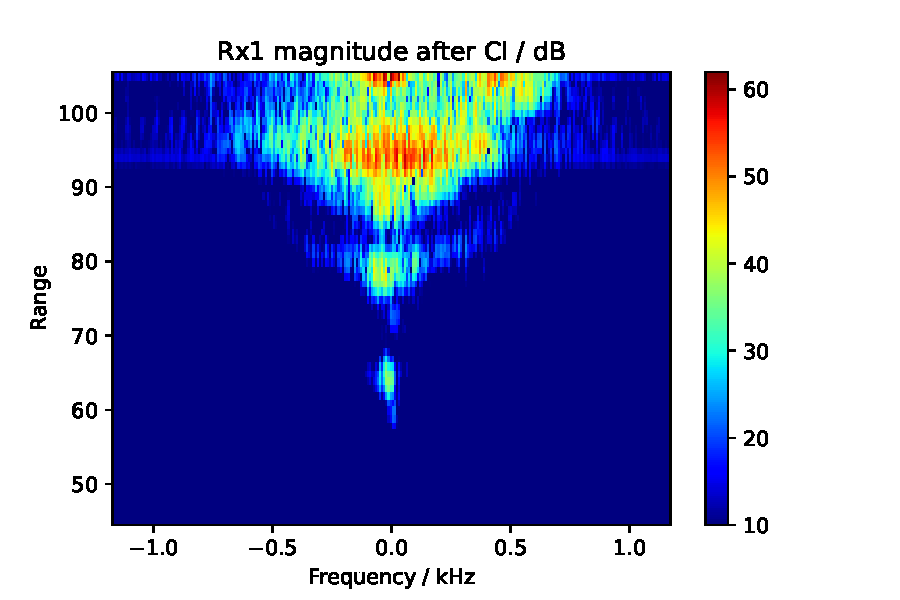
\includegraphics[width=\textwidth]{graphics/t3/t3-mag-rx1.pdf}
    \caption{Task 3: Magnitude of receiver 1 spectrum after 8 CI.}
    \label{fig:t3-mag-x1}
    \end{minipage}\hfill
    \begin{minipage}{0.48\textwidth}
        \centering
             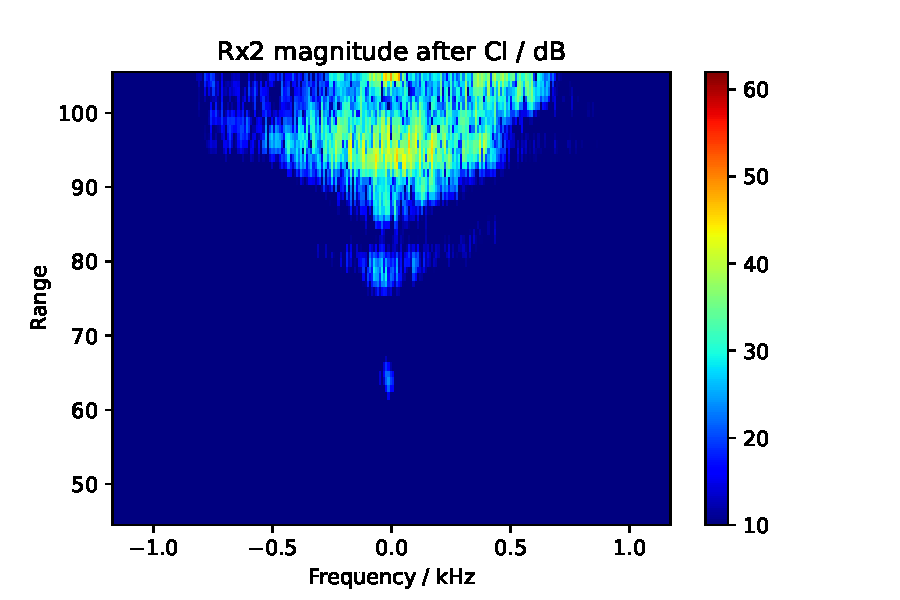
\includegraphics[width=\textwidth]{graphics/t3/t3-mag-rx2.pdf}
    \caption{Task 3: Magnitude of receiver 2 spectrum after 8 CI.}
    \label{fig:t3-mag-rx2}
    \end{minipage}
\end{figure}

\begin{figure}
    \centering
    \begin{minipage}{0.48\textwidth}
        \centering
        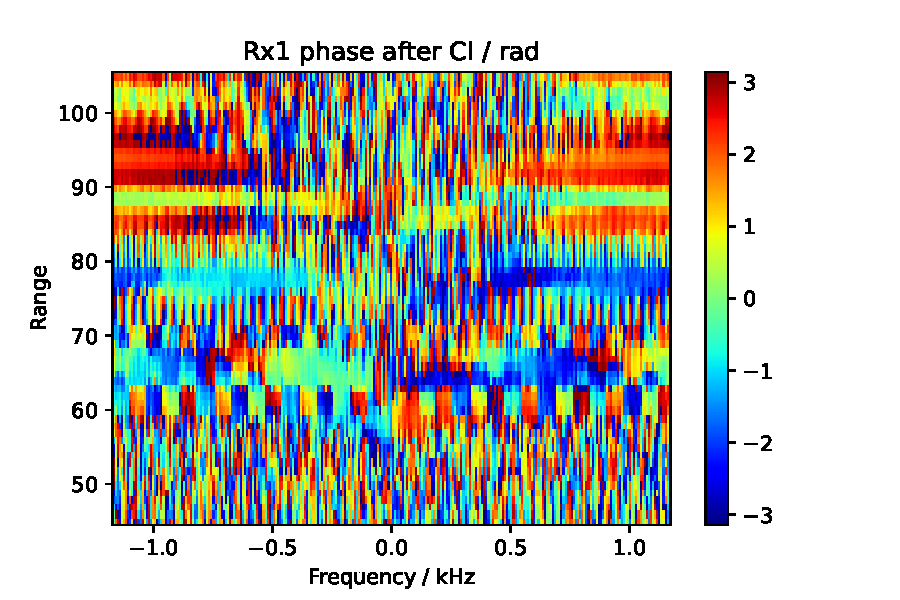
\includegraphics[width=\textwidth]{graphics/t3/t3-phase-rx1.pdf}
    \caption{Task 3: Phase of receiver 1 spectrum after 8 CI.}
    \label{fig:t3-phase-rx1}
    \end{minipage}\hfill
    \begin{minipage}{0.48\textwidth}
        \centering
        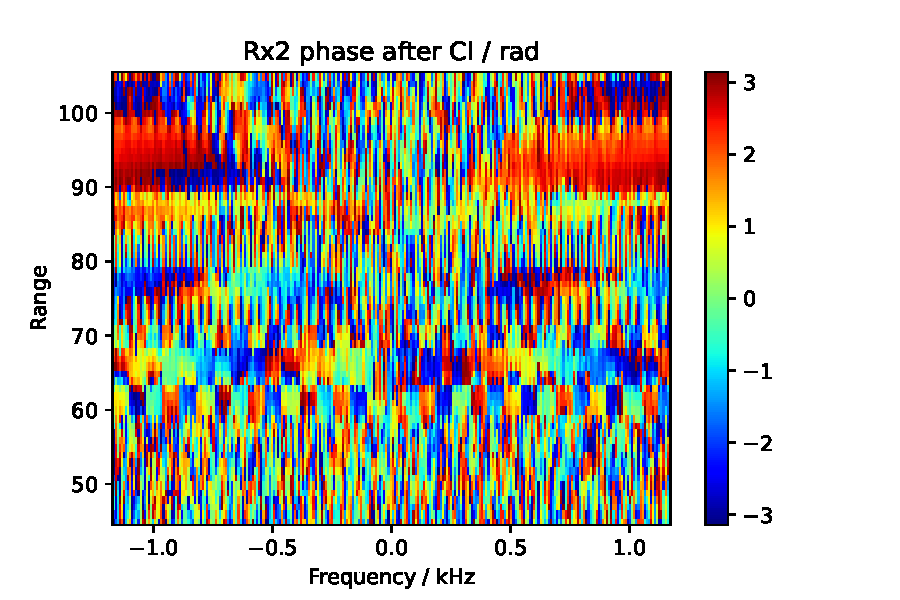
\includegraphics[width=\textwidth]{graphics/t3/t3-phase-rx2.pdf}
    \caption{Task 3: Phase of receiver 2 spectrum after 8 CI.}
    \label{fig:t3-phase-rx2}
    \end{minipage}
\end{figure}
